\documentclass[pdftex,12pt,a4paper]{report}

\usepackage[pdftex]{graphicx}
\usepackage{float}
\usepackage{fancyvrb}
\fvset{xleftmargin=2em}

\usepackage{pgfplots}
\pgfplotsset{width=10cm,compat=1.9}
\usepackage{tikzscale}
\usepackage{pgfplotstable}
\usepackage{booktabs}
\usepackage[font=small,labelfont=bf,tableposition=top]{caption}

\usepackage[utf8]{inputenc} % isto é um comentário
\usepackage[portuges]{babel}
\usepackage[T1]{fontenc}
\usepackage{times}
%\usepackage{lmodern}
\usepackage[obeyspaces,spaces]{url}
\usepackage[left=25mm,right=25mm,top=25mm,bottom=25mm]{geometry}
\usepackage{titlesec}
\usepackage{mathtools}
%identa 1º paragrafo de capitulos e secções
\usepackage{indentfirst}

\newcommand{\HRule}{\rule{\linewidth}{0.5mm}}
\titleformat{\chapter}{\normalfont\huge}{\thechapter.}{20pt}{\huge}


\begin{document}

\begin{titlepage}


\begin{minipage}{0.3\textwidth}
\begin{flushleft} 

\includegraphics[width=\textwidth]{./logo.png}
\end{flushleft}
\end{minipage}
\begin{minipage}{0.6\textwidth}
\begin{flushright} 

\textsc{Departamento de Produção e Sistemas}\\[0.1cm]
\bfseries Mestrado Integrado em Engenharia Informática \\ [0.1cm]
\bfseries \textit{Métodos Determinísticos de Investigação Operacional}\\[8mm]

\end{flushright}
\end{minipage}


\vspace{3cm}


\begin{center}



\textsc{\LARGE Trabalho 1 - Gestão de Projeto}\\[1.5cm]


{\Large \bfseries Grupo 25\\[2cm] }


\begin{minipage}{0.4\textwidth}
	\begin{flushleft} 
		\large Bruno Pereira\\
           Aluno nº 72628 
	\end{flushleft}

\end{minipage}
\begin{minipage}{0.4\textwidth}
	\begin{flushright} 
		\large André Santos\\
           Aluno nº 61778
	\end{flushright}
\end{minipage}

\vfill
\begin{minipage}{0.4\textwidth}
	\begin{center}
		
\large Jéssica Pereira\\
       Aluno nº 71164
	\end{center}

\end{minipage}




\vfill

\large Braga, {\large \today}

\end{center}
\end{titlepage}

\begin{abstract}
Este relatório tem como objetivo apresentar a experiência de modelação
e resolução dos casos propostos na realização do 1º trabalho prático da unidade
curricular de Modelos Determinísticos de Investigação Operacional. Além da
apresentação dos modelos, procuram-se justificar detalhadamente todas as
decisões tomadas. 

O relatório encontra-se dividido por capítulos, em que cada capítulo corresponde
a uma parte do trabalho.
\end{abstract}

\tableofcontents

\chapter{Parte 1}
\label{cap:p1}

\section{Análise do problema}



Neste capítulo, pretende-se criar o modelo do caminho mais longo --- ou caminho
crítico ---, como um modelo de transportes em rede. No problema do caminho
crítico os nós correspondem atividades e a as arestas unidirecionais representam
as precedências entre atividades. Assim, a rede pode ser entendida como um
projeto, no qual as atividades devem ser realizadas obedecendo à ordem das
precedências. De notar que, o caminho mais longo é a duração mínima do projeto.


\begin{figure}[<+htpb+>]
	\centering
	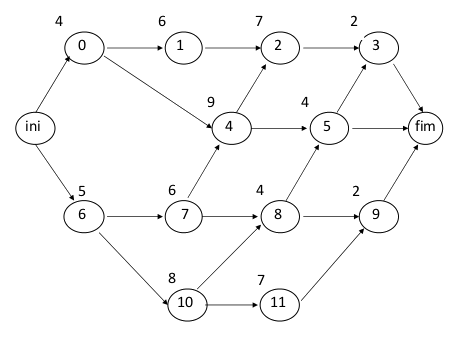
\includegraphics[scale=0.5]{./img/p1_rede_original}
	\caption{Grafo Inicial do enunciado}
\label{p1:fig:rede_original}
\end{figure}

Antes de partir para a formulação do modelo, foi necessário saber qual a rede
a considerar. À rede fornecida no enunciado (figura~\ref{p1:fig:rede_original})
foi necessário retirar dois nós, de acordo com a metodologia apresentada na
secção \textit{Determinação da Lista de Atividades} presente no final do
enunciado. O número de aluno do autor deste relatório é o nº 72628. Logo
o número mais alto é o 72628, então D=2 e E=8, sendo por isso os nodos
2 e 8 a ser retirados da rede. A rede resultante da remoção destes dois nós tem
a representação gráfica mostrada na figura~\ref{p1:fig:rede_com_duracoes}:

\begin{figure}[<+htpb+>]
	\centering
	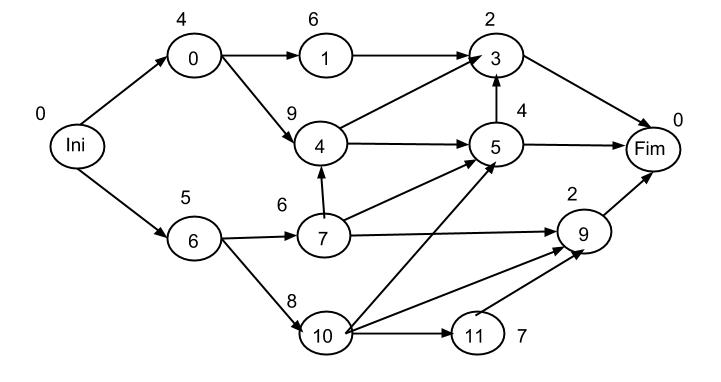
\includegraphics[scale=0.5]{./img/p1_rede_com_duracoes}
	\caption{Grafo resultante da remoção das atividades 2 e 8, com indicação da
	duração de cada atividade (em unidades de tempo arbitrárias)}
\label{p1:fig:rede_com_duracoes}
\end{figure}

\newpage
\section{Modelo}

\subsection{Parâmetros}

Os parâmetros deste modelo são as precedências e as durações de cada atividade,
bem como as capacidades do arco orientado, as ofertas e as procuras em cada
nodo.

\subsection{Variáveis de decisão}
\label{p1:subsec:vardec}


Como já se mencionou anteriormente pretende-se achar o caminho crítico do grafo
orientado. Cada arco terá um valor binário, i.e., 1 caso o arco faça parte do
caminho, 0 caso contrário, considerando que se injeta uma unidade de fluxo no
vértice inicial. Para o efeito, as variáveis de decisão serão nomeadas
$X_{I\_J}$ para a representação dos arcos, tal que a atividade I precede
a atividade J. Assim, $X_{2\_4}$ representa a aresta que vai da atividade 2 para
a atividade 4.

\subsection{Função objetivo}

No caminho mais longo em programação linear, a função objetivo é  uma expressão
que indica a duração de um caminho, onde se pretende que tome o maior valor
possível. Trata-se por isso de um problema de maximização.  Todavia neste
trabalho pretende-se achar o caminho crítico, modelando o problema como um
problema de transportes em rede, ou seja pretende-se minimizar o custo de
transporte, neste caso de uma unidade de fluxo da atividade inicial até à final,
satisfazendo a oferta e a procura em cada nó do grafo. Adiante nesta capítulo
esclarecer-se-á a transformação necessária do primeiro para o segundo modelo.

As variáveis de decisão indicam os arcos que fazem ou não parte de um caminho,
tanto num caso como no outro. A essas variáveis de decisão associaram-se os
custos de cada um dos arcos. Considerou-se que cada arco tem um custo associado
à origem desse arco. Por exemplo, o arco $X_{0\_1}$ tem origem na atividade
0 e destino na atividade 1, e terá um custo de 4, visto ser essa a duração da
atividade 0. Considera-se que a atividade não tem duração para efeitos práticos,
no entanto a passagem de uma atividade para outra passa a assumir a duração.


A função objetivo será o somatório de todos os custos de cada arco multiplicado
pela participação desse arco no caminho crítico. No modelo de programação
linear, para determinar a duração mínima, temos que:

\begin{displaymath}
\max~z = \sum  C_{I\_J} \times X_{I\_J}
\end{displaymath}

Onde:
\begin{description}
	\item[$C_{I\_J}$] Custo associado ao arco que vai de I para J --- parâmetro do problema
	\item[$X_{I\_J}$] Variável de decisão indicativa se o arco faz ou não parte do
	caminho, conforme detalhado na secção~\ref{p1:subsec:vardec}.
\end{description}

Para a transformação deste modelo num modelo de transportes em rede
considerou-se o uso do método simplex dual. A solução com este método
é simétrica da solução do simplex primal. Assim: 

\begin{displaymath}
	\max~z = \sum  C_{I\_J} \times X_{I\_J} \Leftrightarrow - \min -z = \sum
	- C_{I\_J} \times X_{I\_J}
\end{displaymath}




Expandindo a expressão e substituindo os valores de $C_{I\_J}$ pelos valores de
custos do enunciado, juntamente com as variáveis de decisão, temos a seguinte
expressão:

\begin{verbatim}
- min: - 0 Xini_0 - 0 Xini_6 - 4 X0_1 - 4 X0_4
     - 6 X1_3 - 2 X3_fim - 9 X4_3 - 9 X4_5
     - 4 X5_3 - 4 X5_fim - 5 X6_7 - 5 X6_10
     - 6 X7_4 - 6 X7_5 - 6 X7_9 - 2 X9_fim
     - 8 X10_5 - 8 X10_9 - 8 X10_11
     - 7 X11_9;
\end{verbatim}

\subsection{Restrições}
\label{p1:sec:restricoes}

No modelo de transportes em rede as restrições podem ser: restrições de
conservação de fluxo e restrições aos limites superiores e inferiores das
capacidades de cada arco. Dado que para este modelo se considera que uma unidade
de fluxo entra no nodo inicial e sai do nodo final, nada pode permanecer no
grafo, i.e., em cada nó o $fluxo~de~entrada = fluxo~de~saida$.

Assim temos que:

\begin{displaymath}
fluxo~entrada = fluxo~saida \Leftrightarrow  fluxo~entrada - fluxo~saida = 0
\end{displaymath}

Ao ter a equação escrita da segunda forma, considera-se implicitamente o fluxo
de entrada como sendo positivo e o fluxo de saída como negativo, neste caso
1 e -1.

Com a utilização do método simplex dual estas restrições veriam, todos os sinais
a inverterem-se. No entanto, como as todas as restrições são equações e não
inequações, não há nenhum efeito nestas pelo simplex dual. Ou seja, assumamos
o arcos fictícios $Xa\_b$ e $Xb\_c$, numa restrição também fictícia onde $Xa\_b
- Xb\_c = 0$. Com o método dual esta restrição fica como $-Xa\_b + Xb\_c = 0$,
que é equivalente a primeira. Assim $Xa\_b - Xb\_c = 0 \Leftrightarrow -Xa\_b
+ Xb\_c = 0$.

Estas restrições correspondem à procura e oferta em cada nó.

Dado que apenas entra e sai uma unidade de fluxo no grafo, a quantidade que
passa em cada arco será sempre um, pelo que não existe limite superior. Não
obstante, as restrições de não-negatividade serão sempre o limite inferior.

As restrições completas do modelo podem ser vistas na
secção~\ref{p1:sec:fichin}.


\section{Ficheiro \emph{Input}}
\label{p1:sec:fichin}
O ficheiro de \emph{input} é constituído pela função objetivo e restrições, detalhadas
em secções anteriores.

\begin{verbatim}
12                   
20                   
1    2     0     1000 
1    6     0     1000 
6    7    -5     1000 
6   10    -5     1000 
2    4    -4     1000 
2    3    -4     1000 
3    8    -6     1000 
4    5    -9     1000 
4    8    -9     1000 
5    8    -4     1000 
5   12    -4     1000 
7    4    -6     1000 
7    5    -6     1000 
7    9    -6     1000 
10   5    -8     1000 
10  11    -8     1000 
10   9    -8     1000 
11   9    -7     1000 
9   12    -2     1000 
8   12    -2     1000 
1                   
0                    
0                    
0                    
0                    
0                    
0                    
0                    
0                    
0                    
0                    
-1                    

\end{verbatim}

\newpage

\section{\emph{Output} produzido pelo \emph{Relax4}}

O \emph{output} apresentado a seguir foi obtido por \emph{copy-paste} direto
resultante da execução do \emph{Relax4} para
o ficheiro de \emph{input} apresentado anteriormente:

\begin{verbatim}
END OF READING
 NUMBER OF NODES = 12, NUMBER OF ARCS = 20
 CONSTRUCT LINKED LISTS FOR THE PROBLEM
 CALLING RELAX4 TO SOLVE THE PROBLEM
 ***********************************
 TOTAL SOLUTION TIME =  0. SECS.
 TIME IN INITIALIZATION =  0. SECS.
   1 6  1.
   6 7  1.
   4 5  1.
   5 8  1.
   7 4  1.
   8 12  1.
 OPTIMAL COST =  -26.
 NUMBER OF AUCTION/SHORTEST PATH ITERATIONS = 38
 NUMBER OF ITERATIONS =  12
 NUMBER OF MULTINODE ITERATIONS =  1
 NUMBER OF MULTINODE ASCENT STEPS =  0
 NUMBER OF REGULAR AUGMENTATIONS =  2
 ***********************************
\end{verbatim}

\newpage

\section{Resultado}

De acordo com o ficheiro de \emph{output} obtido, o caminho mais longo tem
a duração de 26 unidades de tempo e é o que passa pelas arestas $X_{ini\_6}$,
$X_{6\_7}$, $X_{7\_4}$, $X_{4\_5}$, $X_{5\_3}$ e $X_{3\_fim}$. Em termos
gráficos, o resultado é o apresentado na figura~\ref{p1:fig:caminho_critico}. As
setas de linha cheia indicam as arestas que fazem parte do caminho mais longo,
e os nós por onde esse caminho passa foram colocados a verde.

\begin{figure}[<+htpb+>]
\centering
		  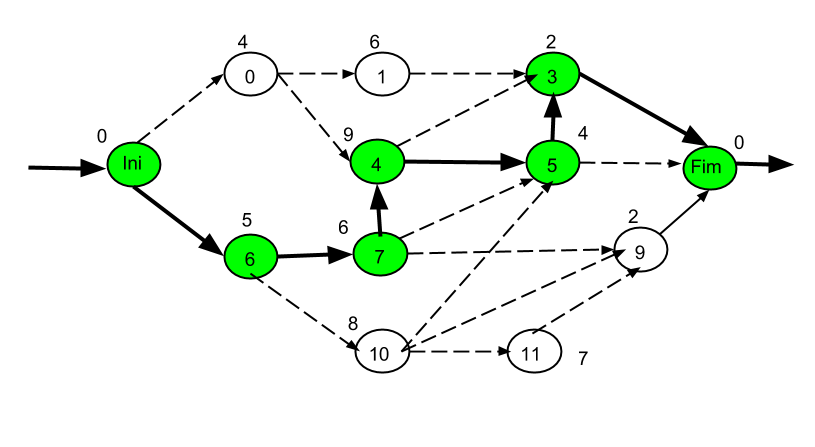
\includegraphics[scale=0.5]{./img/p1_caminho_critico}
\caption{Grafo com indicação do caminho crítico obtido. Os valores em cada nó
representam a duração (em unidades de tempo) da respetiva atividade}
\label{p1:fig:caminho_critico}
\end{figure}

Este resultado indica que as atividades 6,7,4,5 e 3 devem ser vigiadas de perto
e deve-se tentar garantir que são executadas nos tempos previstos, sem atrasos,
caso contrário todo o projeto será atrasado.

\section{Validação do Modelo}

Para validar os resultados, tanto na função objetivo como nas restrições,
substituímos os valores das variáveis de decisão pelo valor que estas tomam na
solução que o lp\_solve indica como ótima. A ideia é verificar que os valores
das variáveis de decisão obtidos confirmam o valor da função objetivo obedecendo
a todas as restrições.

Para evitar ao máximo o erro humano, a substituição de variáveis foi feita
recorrendo a ferramentas que auxiliaram a substituição automática das variáveis
pelo seu valor.

\subsection{Variáveis de Decisão}

No resultado obtido todas as variáveis são de facto binárias, tomam apenas
o valor de 0 ou 1, tal como esperado.

\subsection{Função objetivo}

Depois da substituição das variáveis pelo seu valor, a função objetivo
fica:\\[0.5cm]

$0*0+0*1+4*0+4*0+6*0+2*1+9*0+9*1+4*1+4*0+5*1
+5*0+6*1+6*0+6*0+2*0+8*0+8*0+8*0+7*0 = 26$\\[0.5cm]

Inserindo a expressão numa calculadora verifica-se que a expressão é igual a 26,
o que confirma o resultado obtido com o \textit{lp\_solve}.

\subsection{Restrições}

\begin{itemize}

\item Nodo Inicio 

$1-X_{ini\_6} - X_{ini\_0} = 0$

$1 - 1 - 0 = 0$

\item Nodo 0 

$X_{ini\_0}-X_{0\_1}-X_{0\_4} = 0$

$0 - 0 - 0 = 0$

\item Nodo 1 

$	X_{0\_1}-X_{1\_3} = 0$

$0 - 0 = 0$

\item Nodo 3 

$	X_{1\_3} + X_{4\_3} + X_{5\_3}-X_{3\_fim} = 0$

$0 + 0 + 1 - 1 = 0$

\item Nodo 4 

$	X_{0\_4} + X_{7\_4} - X_{4\_3} - X_{4\_5} = 0$

$0 + 1 - 0 - 1= 0$

\item Nodo 5 

$X_{4\_5} + X_{7\_5} + X_{10\_5} - X_{5\_3} - X_{5\_fim} = 0$

$1 + 0 + 0 - 1 - 0 = 0$

\item Nodo 6 

$X_{ini\_6} - X_{6\_7} - X_{6\_10} = 0$

$1 - 1 - 0 = 0$

\item Nodo 7 

$X_{6\_7}- X_{7\_4}- X_{7\_5} - X_{7\_9} = 0$

$1 - 1 - 0 - 0 = 0$

\item Nodo 9 

$X_{7\_9} + X_{10\_9} + X_{11\_9} - X_{9\_fim} = 0$

$0 + 0 + 0 - 0 = 0$

\item Nodo 10 

$X_{6\_10} - X_{10\_5} - X_{10\_9} - X_{10\_11} = 0$

$0 - 0 - 0 - 0 = 0$

\item Nodo 11 

$X_{10\_11} - X_{11\_9} = 0$

$0 - 0 = 0$

\item Nodo Fim 

$X_{3\_fim} + X_{5\_fim} + X_{9\_fim} - 1 = 0$

$1 + 0 + 0 - 1 = 0$

\end{itemize}

Assim conclui-se que todas as restrições são respeitadas.








\chapter{Parte 2}
\label{cap:p2}

\section{Análise Problema}

O problema do Trabalho 1 tratava da descoberta do tempo em que cada
atividade é iniciada, sabendo que todas as atividades são realizadas.



\section{Modelo Primal --- Trabalho 1}

\subsection{Parâmetros}

Os parâmetros do problema são a duração de cada atividade e as suas
precedências.

\subsection{Variáveis de decisão}

As variáveis de decisão correspondem ao tempo em que cada atividade é iniciada.
Assim, a cada atividade está associada uma variável de decisão. Relativamente ao
nome, a opção tomada foi a de considerar $T_{i}$ como o tempo de início da
atividade $i$ (em unidades de tempo arbitrárias), em que $i$ corresponde ao
número da atividade. Uma vez que apenas se pretende conhecer os tempos de início
de cada atividade, estas são as únicas variáveis deste modelo. 

\subsection{Função Objetivo}

Neste modelo, quer-se minimizar o tempo de execução total do projeto. Isso
corresponde a dizer que queremos que a atividade final seja iniciada o mais cedo
possível. A atividade final é na verdade ``fictícia'', pois não corresponde
a uma atividade que tenha de ser efetivamente realizada. De igual modo,
atividade inicial é  ``fictícia''. No entanto para efeitos de modelação, é útil
considerá-las, para efeitos de modelação do modelo dual. Assume-se que
a atividade final é realizada após todas as outras da rede terem terminado e que
tem duração de 0 unidades de tempo. A atividade inicial tem, de igual modo,
duração de 0 unidades de tempo, sendo pertinente usá-la para a transfonação no
modelo dual.Nestas condições, o tempo inicial da atividade final indica
a duração do projeto.


Uma vez que a variável $T_{fim}$ indica a duração do projeto, a função
objetivo fica simplesmente:

\begin{displaymath} 
	\min~z = T_{fim}-T_{ini} 
\end{displaymath}

\subsection{Restrições}

Com as restrições pretende-se indicar o espaço de possíveis soluções. Sabe-se
que uma atividade não pode começar sem que as que lhe precedem tenham terminado.
Qualquer solução que obedeça a este princípio é uma solução admissível para
o problema. Para escrever as restrições é por isso necessário saber quando uma
atividade termina. Ora, sabendo que as variáveis de decisão usadas indicam
o tempo em que cada atividade se inicia e que se tem a duração das mesmas como
parâmetro do modelo, pode-se dizer que o tempo final de uma atividade
corresponde a somar o seu tempo de início com a sua duração. Ou seja:

\begin{displaymath} Tf_{i} = T_{i} + D_{i} \end{displaymath}

Onde:

\begin{itemize} \item[$Tf_{i}$] Tempo em que a atividade $i$ termina
		\item[$T_{i}$] Tempo em que a atividade i começa (variável de decisão)
		\item[$D_{i}$] Duração da atividade $i$ \end{itemize}

Dizer que uma atividade não pode começar sem que as que lhe precedem tenham
terminado é o mesmo que dizer que o tempo inicial da atividade tem que ser maior
que o tempo final de todas as atividades que lhe precedem. Assumindo que se tem
uma atividade $j$ que precede uma atividade $i$, pode-se escrever que:

\begin{displaymath} T_{i} \geq T_{j} + D_{j} \end{displaymath}

O modelo terá por isso uma restrição deste tipo por cada nodo e por cada
atividade precedente ao nodo. Ou seja, um nó que tenha apenas 1 precedência,
apenas originará uma restrição, enquanto que se o nodo tiver por exemplo
3 precedências, dará origem a 3 restrições --- uma restrição para cada precedência
do nodo. 
As restrições completas:

\begin{itemize}

\item{Nodo Inicial
	\begin{align*}
		T_ {ini} \ge 0 + 0 &         &         &         &         &         &
	\end{align*}}

\item Nodo 0
	\begin{align*}
		T_0 \ge T_{ini} + 0 &         &         &         &         &         &
	\end{align*}


\item Nodo 1
	\begin{align*}
T_1 \ge T_0 + 4 &         &         &         &         &         &
	\end{align*}


\item Nodo 3
\begin{align*}
T_3 \ge T_1 + 6 &         &         &         &         &         &\\
T_3 \ge T_5 + 4 &         &         &         &         &         &\\
T_3 \ge T_4 + 9 &         &         &         &         &         &
	\end{align*}



\item Nodo 4
\begin{align*}
T_4 \ge T_0 + 4 &         &         &         &         &         &\\
T_4 \ge T_7 + 6 &         &         &         &         &         &
	\end{align*}


\item Nodo 5
\begin{align*}
        T_5 \ge T_4 + 9  &         &         &         &         &         &\\
        T_5 \ge T_7 + 6  &         &         &         &         &         &\\
        T_5 \ge T_{10} + 8  &         &         &         &         &         &
	\end{align*}


\item Nodo 6
	\begin{align*}
	T_6 \ge T_{ini} + 0 &         &         &         &         &         &
	\end{align*}

\item Nodo 7
\begin{align*}
       T_7 \ge T_6 + 5  &         &         &         &         &         &\\
	\end{align*}


\item Nodo 9
\begin{align*}
T_9 \ge T_7 + 6   &         &         &         &         &         &\\
T_9 \ge T_{11} + 7 &         &         &         &         &         &\\
T_9 \ge T_{10} + 8 &         &         &         &         &         &
	\end{align*}


\item Nodo 10
\begin{align*}
		T_{10} \ge T_6 + 5 &         &         &         &         &         &
	\end{align*}

\item Nodo 11
\begin{align*}
		T_{11} \ge T_{10} + 8 &         &         &         &         &         &	
\end{align*}



\item Nodo final
\begin{align*}
		T_{fim} \ge T_3 + 2 &         &         &         &         &         &\\
T_{fim} \ge T_5 + 4 &         &         &         &         &         &\\
T_{fim} \ge T_9 + 2 &         &         &         &         &         &
	\end{align*}


\end{itemize}

podem ser consultadas na secção~\ref{p2:sec:ficheiro_input}

Visto que os tempos não podem ser negativos, neste modelo tem-se ainda
restrições de não-negatividade:

\begin{displaymath} T_{i} \geq 0, \forall i_{\in\{ini, 0, 1, 3,
	4,5,6,7,9,10,11,fim\}} \end{displaymath}


\section{Ficheiro \emph{input}}
\label{p2:sec:ficheiro_input}
O ficheiro de \emph{input} é constituído pela função objetivo e restrições, detalhadas
em secções anteriores.

\begin{verbatim}

=== FUNCAO objetivo ===

min: Tfim;


=== RESTRICOES ===

//Nodo Inicial
Tini >= 0 + 0;

//Nodo 0
T0 >= Tini + 0;

//Nodo 1
T1 >= T0 + 4;

//Nodo 3
T3 >= T1 + 6;
T3 >= T5 + 4;
T3 >= T4 + 9;

//Nodo 4
T4 >= T0 + 4;
T4 >= T7 + 6;

//Nodo 5
T5 >= T4 + 9;
T5 >= T7 + 6;
T5 >= T10 + 8;

//Nodo 6
T6 >= Tini + 0;

//Nodo 7
T7 >= T6 + 5;

//Nodo 9
T9 >= T7 + 6;
T9 >= T11 + 7;
T9 >= T10 + 8;

//Nodo 10
T10 >= T6 + 5;

//Nodo 11
T11 >= T10 + 8;

//Nodo final
Tfim >= T3 + 2;
Tfim >= T5 + 4;
Tfim >= T9 + 2;

\end{verbatim}



\newpage
\section{\emph{Output} produzido pelo \texttt{lp\_solve}}

O output apresentado a seguir foi obtido por \emph{copy-paste} direto resultante da execução do \emph{lp\_solve} num sistema linux para o ficheiro de input apresentado anteriormente:

\begin{verbatim} 

\end{verbatim}

\section{Resultado}

O resultado obtido indica uma duração total do projeto de 26 unidades de tempo.
Os tempos iniciais de cada atividade representados graficamente podem ser vistos
na figura~\ref{p2:fig:tempos_inicio}:

\begin{figure}[<+htpb+>] \centering
	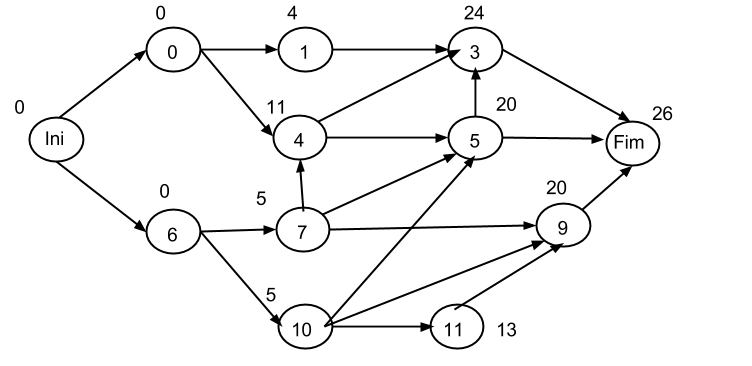
\includegraphics[scale=0.5]{./img/p2_tempos_inicio} \caption{Grafo com
	tempo de início de cada atividade (em unidades de tempo arbitrárias)}
\label{p2:fig:tempos_inicio}
 \end{figure}


\section{Validação do modelo}

Para validar os resultados, tanto na função objetivo como nas restrições,
substituímos os valores das variáveis de decisão pelo valor que estas tomam na
solução que o \texttt{lp\_solve} indica como ótima. A ideia é verificar que os valores das
variáveis de decisão obtidos confirmam o valor da função objetivo obedecendo
a todas as restrições.

Para evitar ao máximo o erro humano, a substituição de variáveis foi feita
recorrendo a ferramentas que auxiliaram a substituição automática das variáveis
pelo seu valor.

\subsection{Variáveis de decisão}

No resultado obtido, todas as variáveis tomam um valor maior ou igual a 0, tal
como seria de esperar.

\subsection{Função objetivo}

Neste modelo a função objetivo consiste apenas no valor de uma variável,
$T_{fim}$, que vale 26 unidades de tempo na solução ótima. Por motivos que não fazem parte do
âmbito deste trabalho, o valor esperado para a duração mínima
do projeto deverá ser o mesmo valor de duração encontrado no caminho crítico da
Parte I. O valor obtido corresponde de facto ao esperado, uma vez que a duração do
caminho crítico obtido na Parte I foi também igual a 26 unidades de tempo.


\subsection{Restrições}


\begin{verbatim} 

//Nodo Inicial
Tini >= 0 + 0;
0 >= 0 + 0;

//Nodo 0
T0 >= Tini + 0; 
0 >= 0 + 0;

//Nodo 1
T1 >= T0 + 4; 
4 >= 0 + 4;

//Nodo 3
T3 >= T1 + 6; 
24 >= 4 + 6;

T3 >= T5 + 4; 
24 >= 20 + 4;

T3 >= T4 + 9; 
24 >= 11 + 9;

//Nodo 4
T4 >= T0 + 4; 
11 >= 0 + 4;

T4 >= T7 + 6; 
11 >= 5 + 6;

//Nodo 5
T5 >= T4 + 9; 
20 >= 11 + 9;

T5 >= T7 + 6; 
20 >= 5 + 6;

T5 >= T10 + 8; 
20 >= 5 + 8;

//Nodo 6
T6 >= Tini + 0; 
0 >= 0 + 0;

//Nodo 7
T7 >= T6 + 5; 
5 >= 0 + 5;

//Nodo 9
T9 >= T7 + 6; 
20 >= 5 + 6;

T9 >= T11 + 7; 
20 >= 13 + 7;

T9 >= T10 + 8; 
20 >= 5 + 8;

//Nodo 10
T10 >= T6 + 5; 
5 >= 0 + 5;

//Nodo 11
T11 >= T10 + 8; 
13 >= 5 + 8;

//Nodo final
Tfim >= T3 + 2; 
26 >= 24 + 2;

Tfim >= T5 + 4; 
26 >= 20 + 4;

Tfim >= T9 + 2; 
26 >= 20 + 2;

\end{verbatim}

Assim conclui-se que todas as restrições são respeitadas.


\chapter{Parte 3}
\label{cap:p3}

\section{Análise do problema}
Nesta 3ª parte do trabalho pretende-se introduzir o conceito do JIT
\emph{just-in-time}. O JIT preconiza a redução das folgas existentes entre
o fim de uma atividade e o início da atividade que a segue. 
As restrições de JIT podem ser generalizadas, para exprimir que o instante de
início da segunda operação deve acontecer num instante de tempo menor ou igual
do que o instante de fim da primeira operação.



\section{Ponto 1}

Considerando o gráfico inicial, pretende-se impor que a atividade 2 comece
imediatamente depois da atividade 1 ter começado, ou seja, $T_2 \le T_1 + D_1$
onde $T_2$ é o tempo da atividade 2, $T_1$ é o tempo da atividade 1 e $D_1$
a duração requerida para a atividade 1. Generalizando $T_j \le T_i + D_i$, onde
$T_j$ é o tempo da atividade j, $T_i$ é o tempo da atividade i e  e $D_1$
a duração requerida para a atividade i., tal que i precede j.

Com esta restrição, podemos achar o caminho mais longo até à atividade 2, para
calcular em seguida o tempo em que atividade 1 pode começar no instante mais
cedo, através da inequação anteriormente referida. Temos que, a duração no arco
da atividade 1 para atividade 2 é igual a 6, que a duração da atividade 1. Então
$T_2 \le T_1 + 6$

Como tal, o caminho mais longo para o nodo 2 é 6->7->4->2, onde as durações
somadas são $T_2 = 5 + 6 + 9 = 20$. Não se considera o tempo da atividade 2 pois esta
ainda não foi realizada. Para obter o valor do $T_1$, temos que $20 \le T_1
+ 6 \Leftrightarrow T_1 \ge 20 - 6 \Leftrightarrow T_1 \ge 14$. Com a restrição
de precedência da atividade 1 com a atividade 2 ($T_2 \ge T_1 + 6$) ficamos com 
$T_1 = 14$, que é o instante mais cedo que a atividade 1 pode começar.

\section{Ponto 2}

As atividades escolhidas do grafo gerado para este trabalho são as atividade
1 e 3. Então $T_3 \le T_1 + D_1 \Leftrightarrow T_3 \le T_1 + 6$. Acrescentou-se
esta restrição no modelo para resolução no \texttt{lp\_solve}, com o mesmo
\emph{output} apresentado na secção anterior, com o acréscimo desta restrição

\newpage

O \emph{output} produzido pelo \texttt{lp\_solve} é o seguinte:

\begin{verbatim}
Value of objective function: 26

Actual values of the variables:
Tfim                           26
T0                              0
Tini                            0
T1                             18
T3                             24
T5                             20
T4                             11
T7                              5
T10                             5
T6                              0
T9                             20
T11                            13

\end{verbatim}


O \emph{output} produzido pelo \texttt{lp\_solve} sem a restrição é o seguinte:

\begin{verbatim}
Value of objective function: 26

Actual values of the variables:
Tfim                           26
T0                              0
Tini                            0
T1                              4
T3                             24
T5                             20
T4                             11
T7                              5
T10                             5
T6                              0
T9                             20
T11                            13

\end{verbatim}

Come se pode ver a atividade 1, ao contrário do modelo do trabalho 1,
adiantou-se para poder cumprir a restrição.


\section{Ponto 3}

Como já foi anteriormente referido nas anteriores secções (Parte I --- descrição
das restrições e Parte II --- passagem das restrições para variáveis de decisão,
neste caso arcos, sendo o modelo primal baseado em nodos), a passagem de uma
restrição no modelo primal para dual passa de uma restrição para um arco, sendo
o arco em questão $X_{3~1}$, a partir da restrição mencionada anteriormente.

\section{Ficheiro de \emph{input} de \emph{Relax4}}


\begin{verbatim}
12                   
21                   
1    2     0     1 
1    6     0     1 
6    7    -5     1 
6   10    -5     1 
2    4    -4     1 
2    3    -4     1 
3    8    -6     1 
4    5    -9     1 
4    8    -9     1 
5    8    -4     1 
5   12    -4     1 
7    4    -6     1 
7    5    -6     1 
7    9    -6     1 
10   5    -8     1 
10  11    -8     1 
10   9    -8     1 
11   9    -7     1 
9   12    -2     1 
8   12    -2     1 
8    3    6      1 -> restrição JIT
1                 
0                    
0                    
0                    
0                    
0                    
0                    
0                    
0                    
0                    
0                    
-1                
\end{verbatim}


\newpage
\section{\emph{Output} produzido pelo \emph{Relax 4}}

\begin{verbatim}
END OF READING
 NUMBER OF NODES = 12, NUMBER OF ARCS = 21
 CONSTRUCT LINKED LISTS FOR THE PROBLEM
 CALLING RELAX4 TO SOLVE THE PROBLEM
 ***********************************
 TOTAL SOLUTION TIME =  0. SECS.
 TIME IN INITIALIZATION =  0. SECS.
   1 6  1.
   6 7  1.
   3 8  1.
   4 5  1.
   5 8  1.
   7 4  1.
   8 12  1.
   8 3  1.
 OPTIMAL COST =  -26.
 NUMBER OF AUCTION/SHORTEST PATH ITERATIONS = 55
 NUMBER OF ITERATIONS =  7
 NUMBER OF MULTINODE ITERATIONS =  1
 NUMBER OF MULTINODE ASCENT STEPS =  1
 NUMBER OF REGULAR AUGMENTATIONS =  1
 ***********************************

\end{verbatim}

\newpage
\section{Resultado}
\label{p3:resultado}


De acordo com o ficheiro de \emph{output} obtido, o caminho mais longo tem
a duração de 26 unidades de tempo (multiplicando por -1, devido ao uso do método
de simplex dual) e é o que passa pelas arestas $X_{ini\_6}$,
$X_{6\_7}$, $X_{7\_4}$, $X_{1\_3}$, $X_{3\_1}$ $X_{4\_5}$, $X_{5\_3}$ e $X_{3\_fim}$. Em termos
gráficos, o resultado é o apresentado na figura~\ref{p3:fig:caminho_critico}. As
setas de linha cheia indicam as arestas que fazem parte do caminho mais longo,
e os nós por onde esse caminho passa foram colocados a verde.

\begin{figure}[<+htpb+>]
	\centering
	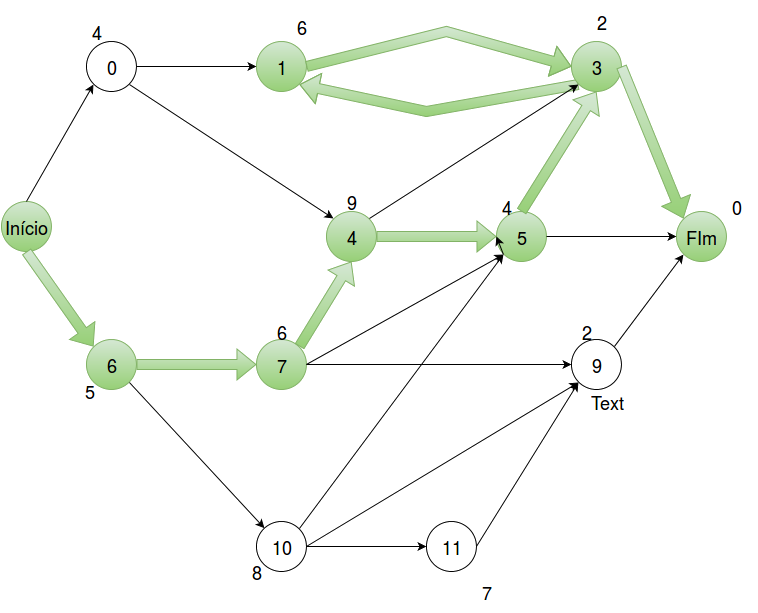
\includegraphics[scale=0.5]{./img/novo_critic}
	\caption{Novo caminho critico}
\label{p3:fig:caminho_critico}
\end{figure}
\section{Validação do modelo}

Para validar os resultados, tanto na função objetivo como nas restrições,
substituímos os valores das variáveis de decisão pelo valor que estas tomam na
solução que o \emph{Relax4} indica como ótima. A ideia é verificar que os valores
das variáveis de decisão obtidos confirmam o valor da função objetivo obedecendo
a todas as restrições.

\subsection{Variáveis de decisão}

No resultado obtido todas as variáveis são de facto binárias, tomam apenas
o valor de 0 ou 1, tal como esperado.


\subsection{Restrições}

\begin{itemize}

\item Nodo Inicio 

$1-X_{ini\_6} - X_{ini\_0} = 0$

$1 - 1 - 0 = 0$

\item Nodo 0 

$X_{ini\_0}-X_{0\_1}-X_{0\_4} = 0$

$0 - 0 - 0 = 0$

\item Nodo 1 


$	X_{0\_1}-X_{1\_3} + X_{3\_1} = 0$

$0 - 1 + 1 = 0$

\item Nodo 3 


$	X_{1\_3} + X_{4\_3} + X_{5\_3}-X_{3\_fim} - X_{3\_1} = 0$

$1 + 0 + 1 - 1 + 1 = 0$

\item Nodo 4 

$	X_{0\_4} + X_{7\_4} - X_{4\_3} - X_{4\_5} = 0$

$0 + 1 - 0 - 1= 0$

\item Nodo 5 

$X_{4\_5} + X_{7\_5} + X_{10\_5} - X_{5\_3} - X_{5\_fim} = 0$

$1 + 0 + 0 - 1 - 0 = 0$

\item Nodo 6 

$X_{ini\_6} - X_{6\_7} - X_{6\_10} = 0$

$1 - 1 - 0 = 0$

\item Nodo 7 

$X_{6\_7}- X_{7\_4}- X_{7\_5} - X_{7\_9} = 0$

$1 - 1 - 0 - 0 = 0$

\item Nodo 9 

$X_{7\_9} + X_{10\_9} + X_{11\_9} - X_{9\_fim} = 0$

$0 + 0 + 0 - 0 = 0$

\item Nodo 10 

$X_{6\_10} - X_{10\_5} - X_{10\_9} - X_{10\_11} = 0$

$0 - 0 - 0 - 0 = 0$

\item Nodo 11 

$X_{10\_11} - X_{11\_9} = 0$

$0 - 0 = 0$

\item Nodo Fim 

$X_{3\_fim} + X_{5\_fim} + X_{9\_fim} - 1 = 0$

$1 + 0 + 0 - 1 = 0$



\end{itemize}


Assim conclui-se que todas as restrições são respeitadas.

\chapter{Parte 4}
\label{cap:p4}

\section{Análise do problema}

O problema deste capítulo baseia-se no modelo apresentado no Capítulo anterior,
e pretende-se encontrar todas as soluções possíveis, a partir da duração inicial
do projeto com várias reduções, de forma a poder relacionar os custos de redução
com o custo do projeto. Desta forma, é possível fazer um balanço de quanto é que
o projeto se pode reduzir e o seu custo de redução. Ou seja, se os custos de
redução justificam a redução pretendida, qual é o máximo que se pode reduzir
e quanto custa.

\section{Modelo}

\subsection{Parâmetros}

À imagem do capítulo anterior, considerou-se a duração de cada atividade
e a suas precedências como parâmetros, bem como os custos de redução e normais
daquelas. Ao contrário das partes anteriores, usou-se os custos normais na construção do modelo. A inclusão deste custos no modelo nesta parte justifica-se pela conveniência no
cálculo dos custos totais em cada unidade que se pretende decrementar, que está
explicado sucintamente mais abaixo neste capítulo.

\subsection{Variáveis de decisão}

As variáveis de decisão são as mesmas que as descritas no Capítulo \ref{cap:p3}, secção
 \ref{p3:vardec}.\ Ou seja, pretende-se decidir qual as reduções necessárias em cada
atividade, com o menor custo total. As reduções são descritas como
anteriormente: 
$$R_i, \forall i \in \{ini, 0, 1, 3, 4,5,6,7,9,10,11,fim\}$$

De igual modo, se inclui os tempos de inicio de atividade, à semelhança do
capítulo anterior:

$$T_i, \forall i \in \{ini, 0, 1, 3, 4,5,6,7,9,10,11,fim\}$$

O significado destas últimas variáveis mantém-se (ver Capítulo \ref{cap:p3}, secção \ref{p3:vardec}).


\subsection{Função Objetivo}
 
A função objetivo sofreu uma modificação em relação ao modelo do capítulo
anterior. Nesta parte, acrescentou-se o custo normal da cada atividade à função objetivo. Assim, a função objetivo agora não representa o custo total suplementar das reduções e passa a representar o custo total do projeto, que engloba os custos normais e os custos suplementares. Continua-se a querer minimizar os custos de redução de forma ótima, apenas se
inclui o custo normal da cada atividade. Note-se que, a soma de todos os custos
normais não influência o valor das variável de decisão (ao contrário dos
custos de redução), uma vez que todas as atividades têm que ser realizadas e os seus custos normais são fixos.
Assim, o valor da função objetivo permite saber o custo total (custos normais
mais custos de redução) para redução de tempo que se pretende efetuar ao projeto.


A função objetivo, para cada atividade $i \in \{ini, 0, 1, 3,
4,5,6,7,9,10,11,fim\}$, é que figura a seguir:

\begin{displaymath} 	
	\min~z = \sum C_{\text{Normal}~i} + C_{\text{Redução}~i} \times R_{i}
\end{displaymath}

Onde:

\begin{itemize} 
	
	\item $C_{\text{Normal}~i}$ --- Custo normal da atividade $i$;

	\item $C_{\text{Redução}~i}$ --- Custo de redução da atividade $i$;
	\item $R_{i}$ --- Redução de tempo da atividade $i$ 

\end{itemize}

Concretizando os valores na função:

\begin{align*}
	\min~z&:&   &400 & +& 100~R0 & +& 1000& +& 300~R1 \\
	      & & + &300 & +& 100~R3 & +& 2000& +& 400~R4 \\
		  & & + &1000& +& 800~R5 & +&  800& +&  90~R6 \\ 
		  & & + &900 & +& 0~R7 & +&  300& +&   0~R9 \\
		  & & + &1600& +& 500~R10& +& 1400& +& 300~R11 \\
\end{align*}

\subsection{Restrições}

As restrições são iguais às da Parte III, com a exceção da restrição do
tempo final do projeto, onde, ao invés de subtrair 3 unidades de tempo ao tempo
do caminho crítico do projeto, considerou-se uma redução gradual (de 1 unidade de tempo) em cada
execução do modelo no \texttt{lp\_solve}, de forma a obter um custo total para
cada valor de redução, e por isso de cada tempo total de execução do projeto. O ponto de partida foi o tempo do projeto obtido na Parte I, de 26 unidades de tempo e a partir dai analisou-se todas as possibilidades redução de tempo até uma redução máxima de 26 unidades de tempo, que corresponde a uma duração nula do projeto. Reduções muito elevadas são impossiveis como seria de esperar, no entanto por uma questão de completudo, consideraram-se todas as possibilidades. Um
\emph{script} em \texttt{BASH} foi criado para o efeito, para executar todos os
modelos. Assim sendo, para cada execução do modelo a restrição do tempo final
fica:

$$ T_{fim} = T_{\text{caminho crítico}} - R_{\text{total desejada}}$$


\begin{itemize} 
	
	\item $T_{fim}$ --- Tempo final;
	\item $T_{\text{caminho crítico}}$ --- Tempo total do caminho crítico;
	\item $R_{\text{total desejada}}$ --- Redução total de tempo desejada no projeto,
		em cada execução do modelo no \texttt{lp\_solve}.

\end{itemize}

Assim:

\begin{align*}	
	 T_{fim}& = 26 - 0 = 26\\
	 T_{fim}& = 26 - 1 = 25\\
	 T_{fim}& = 26 - 2 = 24\\
	 T_{fim}& = 26 - 3 = 23\\
	  \dots     & \\
	 T_{fim}& = 26 - 26 = 0\\
\end{align*}

\section{\emph{Input} do \emph{script} em \emph{BASH}}

O \emph{script} para a execução de cada redução manipula o ficheiro do modelo do
\texttt{lp\_solve}, removendo a última linha onde se encontra a última
restrição, para em seguida adicionar uma nova linha com uma nova restrição
com o novo valor a reduzir. O \emph{output} apresentado corresponde à primeira
linha de cada execução do modelo. O código do \emph{script} foi o seguinte:


\begin{verbatim}
#!/bin/bash

#Nome do ficheiro passado como parâmetro de entrada
file="$1"

#Valor do tempo do caminho crítico
CAM_CRIT=26

#Redução em cada execução
REDUCAO=0
for i in $(seq $CAM_CRIT -1 0)
do
      #Formata string com última restrição com valor da redução
      var='Tfim ='$i';'
      #Elimina a última string do ficheiro
      sed -i '$ d' $file
      #Acrescenta string formatada ao final do ficheiro
      echo $var >> $file
      #Guarda 1ª linha do output de cada execução
      out=$(lp_solve $file | head -n 2) 
      #Apresenta resultado no stdin
      echo Redução de $REDUCAO : $out
      REDUCAO=$((REDUCAO + 1))
done

\end{verbatim}


\newpage

\section{Resultado}

Os valores do \emph{output} da execução do \emph{script} figuram a seguir:

\begin{verbatim}
Redução de 0 (Tfim = 26) : Value of objective function: 9700
Redução de 1 (Tfim = 25) : Value of objective function: 9790
Redução de 2 (Tfim = 24) : Value of objective function: 9880
Redução de 3 (Tfim = 23): Value of objective function: 9980
Redução de 4 (Tfim = 22): Value of objective function: 10380
Redução de 5 (Tfim = 21): Value of objective function: 10780
Redução de 6 (Tfim = 20): Value of objective function: 11180
Redução de 7 (Tfim = 19): Value of objective function: 12280
Redução de 8 (Tfim = 18): This problem is infeasible

\end{verbatim}

Como se pode observar, a partir da redução de 8 unidades de tempo,
o \texttt{lp\_solve} não consegue resolver o modelo, e portanto o output do script a partir dai foi omitido. Logo a redução máxima
possível é de 7 unidades de tempo, que representa realizar o projeto em 19 unidades de tempo, com o custo total de 12280 unidades
monetárias.

A tabela \ref{p4:tab:custos} associa as reduções possíveis ao tempo total do projeto e respetivo custo total de execução do mesmo.

\begin{table}[H]
\centering
\begin{tabular}{c c c}
\toprule
	Redução & Tempo Total & Custos Totais \\ 
\midrule
0&  26& 9700  \\ 
1&  25& 9790  \\
2&  24& 9880  \\
3&  23& 9980  \\
4&  22& 10380 \\
5&  21& 10780 \\
6&  20& 11180 \\
7&  19& 12280 \\
8&  18& $\infty$\\ 
\bottomrule
\end{tabular}
\caption{Reduções em cada execução do modelo no \texttt{lp\_solve}}
\label{p4:tab:custos}
\end{table}

 O gráfico \ref{p4:fig:grafico1} foi elaborado com base na tabela \ref{p4:tab:custos} e mostra o custo total do projeto para cada valor de redução de tempo possíveis.

\begin{figure}[H]
\centering
\resizebox{0.7\textwidth}{!}{%
\begin{tikzpicture}
	\begin{semilogyaxis}
		    [
					x tick label style={/pgf/number format/1000 sep=}, 
	grid=major,
	log ticks with fixed point,
	xlabel={Redução temporal [U.T.]},
	ylabel={Custo Total [U.M.]},
					enlargelimits=0.15, 
			ybar, bar width=7pt, 
				]

\addplot table [x=red,y=custo, color=red,] {data/res.txt};
		\end{semilogyaxis}
\end{tikzpicture}
}%
\caption{Gráfico do custo total do projeto em função das reduções de tempo}
\label{p4:fig:grafico1}
\end{figure}




O gráfico \ref{p4:fig:grafico2} mostra o custo total do projeto para cada valor de duração do projeto.

\begin{figure}[H]
	\centering
	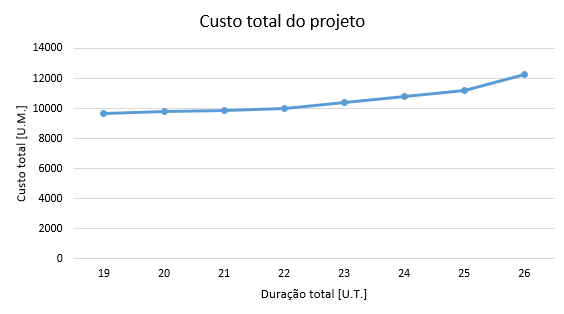
\includegraphics[scale=0.8]{./img/p4_grafico2}
	\caption{Gráfico com custo total em função da duração do projeto}
	\label{p4:fig:grafico2}
\end{figure}

Foram omitidos do gráfico reduções de tempo para as quais não existe solução do modelo.

Os resultados mostram que a duração projeto pode ser reduzida no máximo em 7 unidades  de tempo (duração total de 19 u.t) com um custo total de 12280 unidades monetárias. De igual modo, entre
a duração do projeto sem reduções e redução máxima existem mais 6 possíveis
reduções, com um custo entre 9790 U.T. e 11180 U.M. (não incluindo a máxima
redução).

Através do gráfico \ref{p4:fig:grafico2} é possível perceber os vários compromissos entre a duração total do projeto e o custo total. Nomeadamente, o gráfico sugere que para durações do projeto próximas da inicial (26 unidades de tempo), cada redução adicional não acarreta um aumento nos custos significativo. No entanto, tal já não acontece para durações do projeto mais pequenas, onde cada redução adicional tem custos suplementares elevados. Esse fator pode ser visto no gráfico pelos declives das rectas que unem os vários pontos, que vai aumentando, até ao ponto em que o problema é impossível e não é possível terminar o projeto num tempo menor.

\chapter{Parte 5}
\label{cap:p5}

\section{Análise do problema}

Nesta parte do trabalho pretende-se analisar um cenário semelhante à Parte III, em que se pretende reduzir o tempo total do projeto considerando que é possível reduzir a duração de algumas atividades com um custo suplementar. Na Parte III, o custo suplementar de redução era linear. Nesta parte analisa-se a possibilidade de cada atividade poder ter custos não-lineares quando se reduz a sua duração. Para isso, considera-se uma aproximação a uma função não-linear em que se usam duas funções lineares definidas por ramos. Na prática, corresponde a dizer que cada atividade pode estar sujeita a duas reduções de tipos diferentes, em que cada tipo de redução tem um custo associado. Estes dois tipos de redução serão referidos daqui em diante como reduções do tipo 1 e reduções do tipo 2. Como se trata de uma aproximação a uma função não-linear a partir de duas funções, as reduções do tipo 1 deverão ser aplicadas sempre primeiro que as reduções do tipo 2.

\section{Modelo}

\subsection{Parâmetros}

Nesta parte os parâmetros do problema são as precedências das atividades, as suas durações, o custo de ambos os tipos de redução à duração que se pode fazer e os seus respetivos custos suplementares. Em adição, há limites máximos (em unidades de tempo) para cada tipo de redução possível, sendo esses limites também considerados como parâmetros do problema.

Embora os custos normais das atividades sejam um parâmetro do problema, ele não foi considerado na construção do modelo visto o objetivo deste problema ser o de decidir que reduções de tempo se aplicam às atividades, a um custo suplementar mínimo. Os únicos custos relevantes neste contexto são por isso os custos suplementar de redução apenas, não sendo necessário considerar os custos normais de cada atividade na construção do modelo. Os custos normais da atividade foram apenas considerados na análise dos resultados para o cálculo do custo total do projeto (ver secção \ref{p5:resultado}).

\subsection{Variáveis de decisão}
\label{p5:subsec:vardec}

À semelhança das partes anteriores, também aqui se usou o tempo de início de cada atividade como variáveis de decisão, com a mesma nomenclatura apresentada anteriormente. 

Na Parte III introduziram-se variáveis correspondentes às unidades de tempo a reduzir à duração de cada atividade. Nesta parte, cada atividade tem agora associados dois tipos de reduções possíveis. Cada atividade passa agora a ter associadas duas variáveis de decisão, que traduzem as reduções (em unidades de tempo) do tipo 1 e do tipo 2 a aplicar às durações. A nomenclatura das variáveis para as reduções da Parte III teve que ser alterada aqui, para traduzir precisamente o facto de cada atividade poder ter agora dois tipos de redução possíveis, em vez de apenas 1. As novas variáveis apresentam o seguinte formato:

\begin{displaymath}
R_{i\_j}
\end{displaymath}

Onde:
\begin{itemize}
	\item[$i$] Número da atividade
	\item[$j$] Tipo de redução a aplicar (1 ou 2)
\end{itemize}

Assim, $R_{5\_2}$ representa a redução (em unidades de tempo) do tipo 2 a aplicar à duração da atividade 5.


\subsection{Função objetivo}

A função objetivo deste modelo é uma expressão que representa o custo total suplementar de aplicar reduções de tipo 1 e tipo 2 às durações de todas as atividades.

Na Parte III viu-se que saber o custo suplementar de redução para uma atividade correspondia multiplicar o custo de redução/unidade de tempo pelas unidades de tempo de redução que a atividade sofreu. Nesta parte, há dois tipos de reduções, pelo que para uma atividade $i$ o seu custo suplementar de redução total, $C_{i}$, será dado por:

\begin{displaymath}
C_{i} = C_{i\_1} \times R_{i\_1} + C_{i\_2} \times R_{i\_2}
\end{displaymath}

Onde:

\begin{itemize}
	\item[$C_{i\_1}$] Custo por unidade de tempo associada a reduções do tipo 1 na duração da atividade $i$
	\item[$R_{i\_1}$] Unidades de tempo reduzir à duração da atividade $i$ a custo $C_{i\_1}$
	\item[$C_{i\_2}$] Custo por unidade de tempo associada a reduções do tipo 2 na duração da atividade $i$
	\item[$R_{i\_2}$] Unidades de tempo reduzir à duração da atividade $i$ a custo $C_{i\_2}$
\end{itemize}

A função objetivo, $z$, corresponde ao somatório dos custos de redução de todas as atividades, ou seja:

\begin{displaymath}
min~z = \sum C_i
\end{displaymath}

Substituindo os custos das reduções de cada tipo pelo valor dado no enunciado, ficamos com a seguinte função objetivo:

\begin{verbatim}
min: 100 R0_1 + 200 R0_2 + 300 R1_1 + 600 R1_2 + 100 R3_1 + 200 R3_2 + 
400 R4_1 + 800 R4_2 + 800 R5_1 + 1600 R5_2 + 90 R6_1 + 180 R6_2 + 
0 R7_1 + 0 R7_2 + 0 R9_1 + 0 R9_2 + 500 R10_1 + 1000 R10_2 + 300 R11_1 
+ 600 R11_2;
\end{verbatim}


\subsection{Restrições}

Também as restrições serão muito semelhantes às da Parte III.
Em primeiro lugar, mantêm-se as restrições referentes às unidades de tempo máximas que se pode reduzir. Assim cada variável de decisão relativa às reduções a aplicar, terá uma restrição a limitar o seu valor máximo. Visto cada atividade poder estar sujeita a 2 tipos de redução, por cada atividade ter-se-á então 2 restrições relativas aos limites máximos de redução. Em termos genéricos, para a atividade $i$, essas duas restrições podem ser escritas como:

\begin{displaymath}
R_{i\_1} \leq Rmax_{i\_1}; R_{i\_2} \leq Rmax_{i\_2}
\end{displaymath}

Onde:

\begin{itemize}
	\item[$R_{i\_1}$] Variável de decisão --- redução (em unidades de tempo) do tipo 1 a aplicar à atividade $i$
	\item[$R_{i\_2}$] Variável de decisão --- redução (em unidades de tempo) do tipo 2 a aplicar à atividade $i$
	\item[$Rmax_{i\_1}$] Redução máxima de tempo do tipo 1 que é possível aplicar à atividade $i$
	\item[$Rmax_{i\_2}$] Redução máxima de tempo do tipo 2 que é possível aplicar à atividade $i$
\end{itemize}

Por exemplo, para a atividade 5 tem-se as seguintes restrições:

\begin{verbatim}
R5_1 <= 0.5;
R5_2 <= 0.5;
\end{verbatim}

Tal como na Parte III, também as restrições relativas aos tempos de inicio de cada atividade estão presentes neste modelo. Recorde-se que na Parte III tais restrições tinham o seguinte aspecto:

\begin{displaymath}
T_{i} \leq T_{j} + (D_{j} - R{j})
\end{displaymath}

\begin{itemize}
	\item[$T_{i}$] Tempo em que a atividade $i$ inicia
	\item[$T_{j}$] Tempo em que a atividade $j$ inicia
	\item[$D_{j}$] Duração da atividade $j$
	\item[$R_{j}$] Redução de tempo a aplicar na atividade $j$
\end{itemize}

A inequação apresentada em cima parte tem como pressuposto a atividade $j$ preceder a atividade $i$.
A diferença introduzida no modelo desta parte é que cada atividade pode agora ter dois tipos de redução possíveis, pelo que as restrições têm que contar com esse novo fator. Nas restrições da Parte III, o facto de cada atividade poder ver reduzida a sua duração está patente na parcela $(D_{j} - R{j})$ no segundo membro da inequação. Seguindo uma lógica semelhante, dizer que uma atividade pode contar com dois tipos de redução, corresponde a dizer a subtrair uma nova redução à duração. Ou seja:

\begin{displaymath}
T_{i} \leq T_{j} + (D_{j} - R{j\_1} - R{j\_2})
\end{displaymath}

\begin{itemize}
	\item[$R_{j\_1}$] Redução (em unidades de tempo) do tipo 1 a aplicar na atividade $j$
	\item[$R_{j\_2}$] Redução (em unidades de tempo) do tipo 2 a aplicar na atividade $j$
\end{itemize}

Neste modelo era também necessário forçar um tempo de duração total do projeto. Tal como na Parte III, isso foi feito forçando a variável $T_{fim}$ a tomar um valor concreto. Neste modelo usou-se a mesma ideia. Pedia-se que o tempo total do projeto neste modelo fosse inferior em 4 unidades de tempo ao obtido na Parte I. Na Parte I, o tempo total do projeto foi de 26 unidades de tempo. Assim, a restrição que força o tempo total do projeto é:

\begin{verbatim}
Tfim = 26-4;
\end{verbatim}

Visto que os tempos e as reduções não podem ser negativos, neste modelo tem-se ainda restrições de não-negatividade:

\begin{displaymath}
T_{i} \geq 0;  R_{i\_1} \geq 0; R_{i\_2} \geq 0; \forall i_{\in\{ini, 0, 1, 3, 4,5,6,7,9,10,11,fim\}}
\end{displaymath}


\section{Ficheiro \emph{Input}}
\label{p5:sec:fichin}

\begin{verbatim}
/*
=== FUNCAO OBJECTIVO ===
Minimizar os custos suplementares de redução das atividades.
*/
min: 100 R0_1 + 200 R0_2 +
300 R1_1 + 600 R1_2 +
100 R3_1 + 200 R3_2 +
400 R4_1 + 800 R4_2 +
800 R5_1 + 1600 R5_2 +
90 R6_1 + 180 R6_2 +
0 R7_1 + 0 R7_2 +
0 R9_1 + 0 R9_2 +
500 R10_1 + 1000 R10_2 +
300 R11_1 + 600 R11_2;


/*
Reducoes maximas
*/
R0_1 <= 0.5;
R0_2 <= 0.5;

R1_1 <= 1;
R1_2 <= 1;

R3_1 <= 0.5;
R3_2 <= 0.5;

R4_1 <= 1;
R4_2 <= 1;

R5_1 <= 0.5;
R5_2 <= 0.5;

R6_1 <= 1;
R6_2 <= 1;

R7_1 <= 0;
R7_2 <= 0;

R9_1 <= 0;
R9_2 <= 0;

R10_1 <= 0.5;
R10_2 <= 0.5;

R11_1 <= 1;
R11_2 <= 1;


//Nodo Inicial
Tini >= 0 + 0;
//Nodo 0
T0 >= Tini + 0 - Rini;
//Nodo 1
T1 >= T0 + 4 - R0_1 - R0_2;
//Nodo 3
T3 >= T1 + 6 - R1_1 - R1_2;
T3 >= T5 + 4 - R5_1 - R5_2;
T3 >= T4 + 9 - R4_1 - R4_2;
//Nodo 4
T4 >= T0 + 4 - R0_1 - R0_2;
T4 >= T7 + 6 - R7_1 - R7_2;
//Nodo 5
T5 >= T4 + 9 - R4_1 - R4_2;
T5 >= T7 + 6 - R7_1 - R7_2;
T5 >= T10 + 8 - R10_1 - R10_2;
//Nodo 6
T6 >= Tini + 0 - Rini;
//Nodo 7
T7 >= T6 + 5 - R6_1 - R6_2;
//Nodo 9
T9 >= T7 + 6 - R7_1 - R7_2;
T9 >= T11 + 7 - R11_1 - R11_2;
T9 >= T10 + 8 - R10_1 - R10_2;
//Nodo 10
T10 >= T6 + 5 - R6_1 - R6_2;
//Nodo 11
T11 >= T10 + 8 - R10_1 - R10_2;
//Nodo final
Tfim >= T3 + 2 - R3_1 - R3_2;
Tfim >= T5 + 4 - R5_1 - R5_2;
Tfim >= T9 + 2 - R9_1 - R9_2;

/*Forcar reducao de tempo*/
Tfim = 26-4;
\end{verbatim}



\section{\emph{Output} produzido pelo \texttt{lp\_solve}}

\begin{verbatim}
Value of objective function: 820

Actual values of the variables:
R0_1                            0
R0_2                            0
R1_1                            0
R1_2                            0
R3_1                          0.5
R3_2                          0.5
R4_1                            1
R4_2                            0
R5_1                            0
R5_2                            0
R6_1                            1
R6_2                            1
R7_1                            0
R7_2                            0
R9_1                            0
R9_2                            0
R10_1                           0
R10_2                           0
R11_1                           0
R11_2                           0
Tini                            0
T0                              0
Rini                            0
T1                              4
T3                             21
T5                             17
T4                              9
T7                              3
T10                             3
T6                              0
T9                             18
T11                            11
Tfim                           22
\end{verbatim}

\section{Resultado}
\label{p5:resultado}

Os resultados do lpsolve mostram que se consegue reduzir a duração total do projeto em 4 unidades de tempo, passando o projeto a demorar 22 unidades de tempo, com um custo suplementar de 820 unidades monetárias.

O custo total do projeto é dado pela soma dos custos normais das atividades com os custos suplementares de redução às suas durações, sendo este último valor o resultado obtido na função objetivo. O custo normal das atividades é:

\begin{displaymath}
400+1000+300+2000+1000+800+900+300+1600+1400 = 9700~u.m.
\end{displaymath}

O custo total do projeto é dado pela soma dos custos normais das atividades com os custos suplementares de redução às suas durações, sendo este último valor o resultado obtido na função objetivo. Assim, o projeto tem a duração de 22 unidades de tempo, com um custo total de $9700 + 820 = 10520~u.m.$.

O grafo da figura \ref{p5:fig:tempos_inicio} mostra os novos tempos iniciais de cada atividade de acordo com o resultado obtido no lpsolve:

\begin{figure}[<+htpb+>]
	\centering
	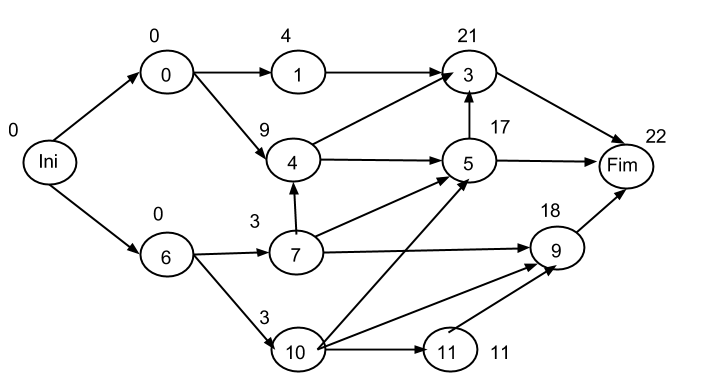
\includegraphics[scale=0.5]{./img/p5_tempos_inicio}
	\caption{Grafo com tempos de inicio das atividades}
	\label{p5:fig:tempos_inicio}
\end{figure}

A figura \ref{p5:fig:reducoes} apresenta o mesmo grafo, com indicação das reduções feitas às atividades e respetivas durações. Os números a roxo indicam as reduções de tipo 1 e os números a verde as reduções de tipo 2.

\begin{figure}[<+htpb+>]
	\centering
	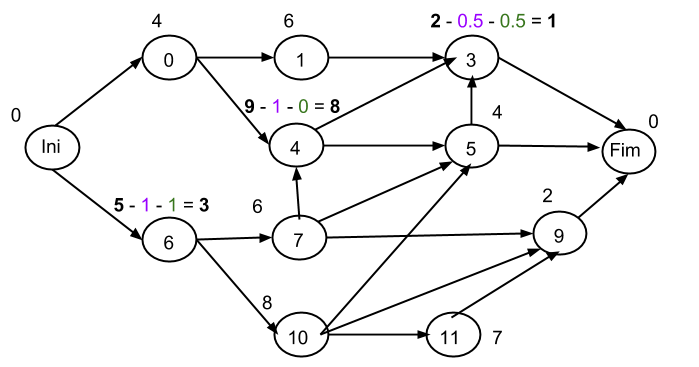
\includegraphics[scale=0.5]{./img/p5_reducoes}
	\caption{Grafo com reduções de tempo às atividades}
	\label{p5:fig:reducoes}
\end{figure}

O Diagrama de Gantt correspondente à execução do projeto encontra-se na figura \ref{p5:fig:diagrama_gantt}:

\begin{figure}[<+htpb+>]
	\centering
	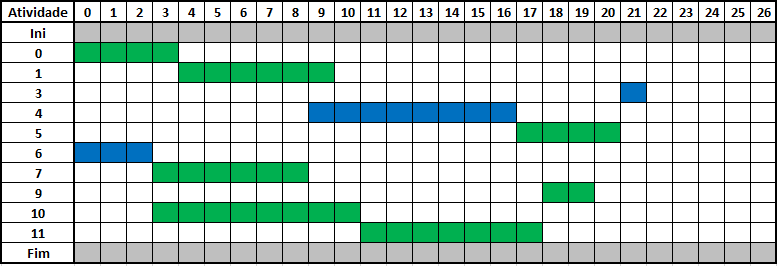
\includegraphics[scale=0.5]{./img/p5_diagrama_gantt}
	\caption{Grafo com reduções de tempo às atividades}
	\label{p5:fig:diagrama_gantt}
\end{figure}

As atividades que sofreram redução encontram-se marcadas a azul.

É interessante também notar que a duração total do projeto é de 22 unidades de tempo, no entanto, se somarmos as novas durações das atividades que na Parte I faziam parte do caminho crítico tem-se uma duração de $3+6+8+1=18$ unidades de tempo. Visto que a duração do projeto não é a mesma do caminho crítico da Parte I, podemos concluir que o caminho crítico se alterou com as reduções aplicadas.

\section{Validação do Modelo}

Para validar os resultados, tanto na função objetivo como nas restrições,
substituímos os valores das variáveis de decisão pelo valor que estas tomam na
solução que o lp\_solve indica como ótima. A ideia é verificar que os valores das
variáveis de decisão obtidos confirmam o valor da função objetivo obedecendo
a todas as restrições.

Para evitar ao máximo o erro humano, a substituição de variáveis foi feita
recorrendo a ferramentas que auxiliaram a substituição automática das variáveis
pelo seu valor.

\subsection{Variáveis de Decisão}

No resultado obtido, todas as variáveis tomam um valor maior ou igual a 0, tal
como seria de esperar.

\subsection{Função objetivo}

Depois da substituição das variáveis pelo seu valor, a função objetivo
fica:\\

$100*0+200*0+300*0+600*0+100*0.5+200*0.5+400*1+800*0+800*0+
1600*0+90*1+180*1+0*0+0*0+0*0+0*0+500*0+1000*0+300*0+600*0$\\

Inserindo a expressão numa calculadora verifica-se que a expressão é igual a 820,
o que confirma o resultado obtido com o \textit{lp\_solve}.

\subsection{Restrições}

\begin{verbatim}

/*
Reducoes maximas
*/
R0_1 <= 0.5;
R0_2 <= 0.5;

0 <= 0.5;
0 <= 0.5;


R1_1 <= 1;
R1_2 <= 1;

0 <= 1;
0 <= 1;

R3_1 <= 0.5;
R3_2 <= 0.5;

0.5 <= 0.5;
0.5 <= 0.5;

R4_1 <= 1;
R4_2 <= 1;

1 <= 1;
0 <= 1;

R5_1 <= 0.5;
R5_2 <= 0.5;

0 <= 0.5;
0 <= 0.5;

R6_1 <= 1;
R6_2 <= 1;

1 <= 1;
1 <= 1;


R7_1 <= 0;
R7_2 <= 0;

0 <= 0;
0 <= 0;

R9_1 <= 0;
R9_2 <= 0;

0 <= 0;
0 <= 0;


R10_1 <= 0.5;
R10_2 <= 0.5;

0 <= 0.5;
0 <= 0.5;


R11_1 <= 1;
R11_2 <= 1;

0 <= 1;
0 <= 1;



//Nodo Inicial
Tini >= 0 + 0;
0 >= 0 + 0;
//Nodo 0
T0 >= Tini + 0 - Rini;
0 >= 0 + 0 - 0;
//Nodo 1
T1 >= T0 + 4 - R0_1 - R0_2;
4 >= 0 + 4 - 0 - 0;
//Nodo 3
T3 >= T1 + 6 - R1_1 - R1_2;
T3 >= T5 + 4 - R5_1 - R5_2;
T3 >= T4 + 9 - R4_1 - R4_2;

21 >= 4 + 6 - 0 - 0;
21 >= 17 + 4 - 0 - 0;
21 >= 9 + 9 - 1 - 0;
//Nodo 4
T4 >= T0 + 4 - R0_1 - R0_2;
T4 >= T7 + 6 - R7_1 - R7_2;
9 >= 0 + 4 - 0 - 0;
9 >= 3 + 6 - 0 - 0;
//Nodo 5
T5 >= T4 + 9 - R4_1 - R4_2;
T5 >= T7 + 6 - R7_1 - R7_2;
T5 >= T10 + 8 - R10_1 - R10_2;
17 >= 9 + 9 - 1 - 0;
17 >= 3 + 6 - 0 - 0;
17 >= 3 + 8 - 0 - 0;
//Nodo 6
T6 >= Tini + 0 - Rini;
0 >= 0 + 0 - 0;
//Nodo 7
T7 >= T6 + 5 - R6_1 - R6_2;
3 >= 0 + 5 - 1 - 1;
//Nodo 9
T9 >= T7 + 6 - R7_1 - R7_2;
T9 >= T11 + 7 - R11_1 - R11_2;
T9 >= T10 + 8 - R10_1 - R10_2;
18 >= 3 + 6 - 0 - 0;
18 >= 11 + 7 - 0 - 0;
18 >= 3 + 8 - 0 - 0;
//Nodo 10
T10 >= T6 + 5 - R6_1 - R6_2;
3 >= 0 + 5 - 1 - 1;
//Nodo 11
T11 >= T10 + 8 - R10_1 - R10_2;
11 >= 3 + 8 - 0 - 0;
//Nodo final
Tfim >= T3 + 2 - R3_1 - R3_2;
Tfim >= T5 + 4 - R5_1 - R5_2;
Tfim >= T9 + 2 - R9_1 - R9_2;
22 >= 21 + 2 - 0.5 - 0.5;
22 >= 17 + 4 - 0 - 0;
22 >= 18 + 2 - 0 - 0;

/*Forcar reducao de tempo*/
Tfim = 26-4;
22 = 26-4;

\end{verbatim}

Assim conclui-se que todas as restrições são respeitadas.












\end {document}


